\section{System}
\begin{figure*}[t]
\centering
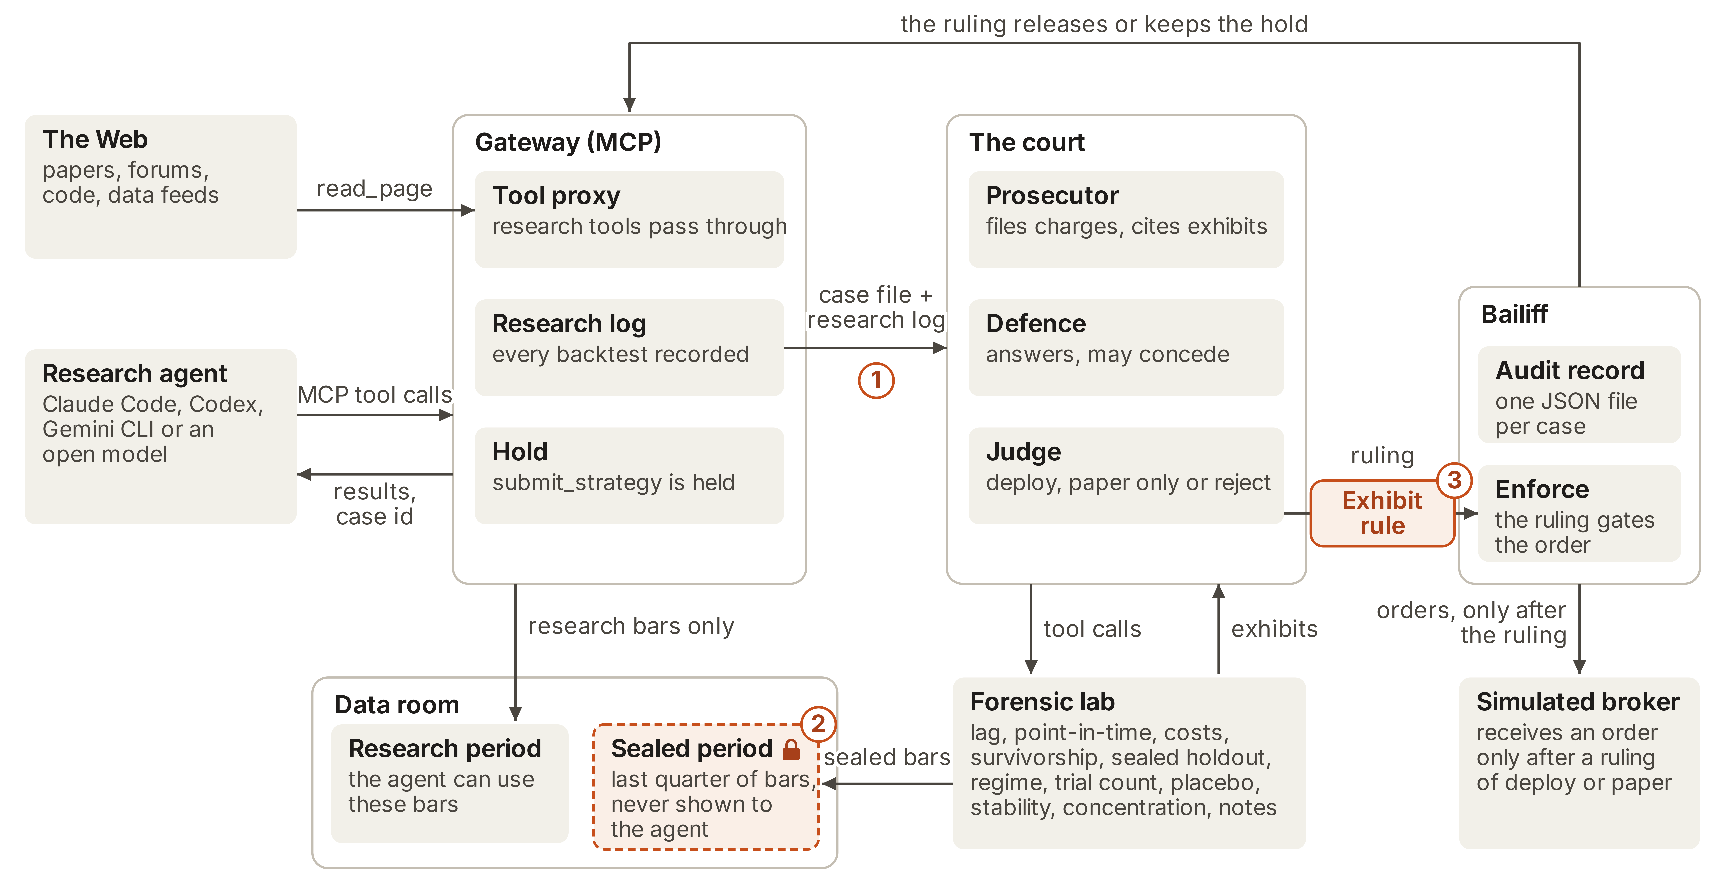
\includegraphics[width=\textwidth]{fig_architecture.pdf}\\[2pt]
\IfFileExists{fig_trial_strip.pdf}{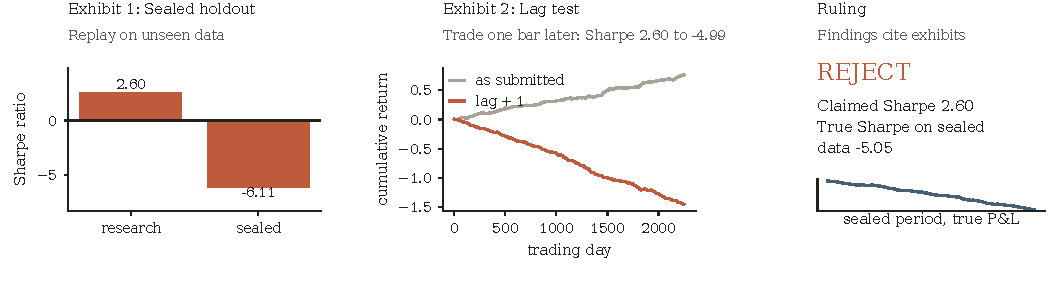
\includegraphics[width=\textwidth]{fig_trial_strip.pdf}}{\fbox{\parbox[c][1.75in][c]{0.97\textwidth}{\centering\sffamily Placeholder for the trial strip: two exhibits with their charts, and the ruling.}}}
\caption{AlphaCourt. Top: the agent reaches the Web and data room only through the gateway, which logs backtests and holds requests for capital. The court works from exhibits made by the forensic lab, which alone reads the sealed period. The exhibit rule strikes findings that cite no damaging exhibit. The bailiff orders the simulated broker only after a ruling of deploy or paper. Bottom: one trial of a guilty case, a look-ahead strategy from the dev split (a demonstration case, not typical). The agent claimed a Sharpe of 2.60. On the sealed period, in the one world replayed, it scores -6.11, and -4.99 with one more bar of delay, so the court rejects it. Its true edge, averaged over fresh worlds, is -5.05. The small curve is the true profit on sealed data, shown only after the ruling.} % source: web/public/data/cases/AC-D014-G.json (claim 2.60; holdout_test -6.11; lag_test -4.99; truth.sharpe -5.0546; ruling reject)
\Description{Top: a boxes-and-arrows diagram. A research agent and the Web connect to a gateway box that holds a tool proxy, a research log and a hold. The gateway passes a case file and the log to a court box with a prosecutor, a defence and a judge. A forensic lab box exchanges tool calls and exhibits with the court and reads a sealed period in the data room. The judge's ruling passes through an exhibit rule to a bailiff box that writes an audit record and enforces the ruling on a simulated broker. Bottom: a bar chart of the Sharpe ratio in research and on sealed data, a line chart of cumulative return as submitted and with a one-bar delay, and a box giving the ruling, reject, with the claimed and true Sharpe ratios.}
\label{fig:system}
\end{figure*}

AlphaCourt has three parts: a gateway, a data room and a court. Figure~\ref{fig:system} shows how they connect.

\paragraph{The gateway.}
A research agent reaches AlphaCourt over MCP~\cite{mcp2025}, through six tools: \texttt{list\_fields}, \texttt{field\_info}, \texttt{read\_page}, \texttt{run\_backtest}, \texttt{submit\_strategy} and \texttt{get\_verdict}. % source: gateway/mcp.py TOOLS (six tools)
Research calls pass through and are logged, each backtest with a hash of its specification.
\texttt{submit\_strategy} deploys nothing. It returns a case number with the status ``held''.
A strategy is a JSON specification (a signal formula in a small whitelisted language, a lag, a universe, costs), never free code, so every test can re-run it.

\paragraph{The data room and the sealed period.}
The agent trades in a simulated market of 300 assets and 3,000 daily bars. % source: court/market.py make_world(T=3000, N=300)
Returns carry planted effects of known size, and delistings follow bad returns.
Some fields leak the future on purpose, such as restated earnings; \texttt{field\_info} documents when each is available.
The last quarter of the bars is sealed. % source: court/market.py research_end = int(0.75 * T)
Research tools never return it; only the forensic lab reads it.
The \emph{true edge} of a strategy is its Sharpe ratio on the sealed period, computed under strict point-in-time data, a lag of at least one bar, the full universe including delisted assets, and realistic costs, averaged over fresh worlds with the same parameters. No model is involved.

\paragraph{The forensic lab.}
Eleven deterministic tests each return an \emph{exhibit}: a numbered record with the test, its parameters, its numbers, a hint (damaging, neutral or supportive, from fixed thresholds) and chart data. % source: court/forensics.py TOOLS (eleven tests)
The tests re-run the strategy with one more bar of delay, with strict point-in-time data, at higher costs, on the full universe and on the sealed period. They split performance by regime and year, shuffle the signal as a placebo, scan the notes and pages read for text addressed to reviewers, and correct for the number of trials~\cite{bailey2014}.
The tests are standard practice; none is new. The trial-count test counts backtests in the gateway's log, not the agent's report.

\paragraph{The court and the exhibit rule.}
A clerk (plain code) builds the case file: the specification, the claim, the log summary and the pages read.
The prosecutor, a language model, may run up to six tests and files charges that each cite exhibit numbers. % source: court/trial.py DEFAULT_BUDGET prosecutor_tools
The defence may run up to four tests, answer each charge and concede. % source: court/trial.py DEFAULT_BUDGET defence_tools
The judge reads the exhibits, charges and rebuttals and rules deploy, paper trading only, or reject, with a verdict on each charge and an opinion of at most 120 words. % source: court/roles.py JUDGE_SYSTEM
Plain code applies the \emph{exhibit rule} after the judge rules. A charge the judge upholds is struck unless it cites a damaging exhibit, a test the strategy failed. If no charge survives a paper or reject ruling, the ruling becomes deploy and is flagged \emph{unsupported}. % source: court/trial.py apply_exhibit_rule
The rule checks that a damaging exhibit is cited, not that it fits the charge.

\paragraph{The bailiff.}
The gateway enforces the ruling. Deploy books capital to a simulated account, paper books it as paper capital, and reject books nothing; a trial that fails also books nothing. % source: gateway/broker.py, gateway/service.py _work
The record is a JSON audit file per case with the submission, charges, exhibits, rebuttal, verdict and model identifiers, written before the case is marked final. % source: gateway/audit.py, gateway/service.py _work
The broker is an in-memory data structure; no order is ever sent.
